\documentclass[12pt]{article}

\usepackage{minted}
\usemintedstyle{emacs}
\usepackage{cite}
\usepackage[pdftex]{graphicx}
\usepackage{subcaption}
%\usepackage{amsmath}
%\usepackage[table,x11names]{xcolor}

%\usepackage[margin=1.25in]{geometry}
\usepackage[onehalfspacing]{setspace}

%opening
\title{LIN5022 Grammar Models\\Dependency Grammars}
\author{Thuong-Hai Pham}

\begin{document}

\maketitle

In the scope of this report, we will discuss about the basic concepts and terminologies being used to constitute the Dependency Grammar in section \ref{basic}. Thereafter, we clarify the head-dependant criteria in section \ref{head_dep} followed by formal conditions and properties of dependency graph in section \ref{dg_graph}. To end with the review of Dependency Grammar, four dimensions in variant space is discussed in detail within section \ref{dg_var}. Finally, we review different approaches for the problem of dependency parsing.

\section{Dependency Grammar}

\subsection{Basic concepts \& terminologies} \label{basic}
In fact, Dependency Grammar is not a single consistently established grammar, yet a wide range of variants that share several basic assumptions. The primary underlying idea is the syntactic structure which consists of lexical items, connected by binary asymmetric relations. These relations are called dependencies. Although it is said that this concept had been used early in Panini's work for Sanskrit grammar around $6^{th}$ to $4^{th}$ century BCE, we can consider the starting point at the time when it were introduced systematically by \cite{tesniere1959elements} as quoted in his work (translated to English by \cite{nivre2005dependency})
\begin{quote}
	The sentence is an organised whole, the constituent elements of which are words. Every word that belongs to a sentence ceases by itself to be isolated as in the dictionary. Between the word and its neighbours, the mind perceives connections, the totality of which forms the structure of the sentence. The structural connections establish dependency relations between the words. Each connection in principle unites a superior term and an inferior term. The superior term receives the name governor. The inferior term receives the name subordinate.
\end{quote}

As quoted above, the two parties involved in this type of relation are called governor and subordinate. In literature, the governor can be also called by other names, most popular as head, or regent. While the subordinate is dependant, or modifier.

Figure \ref{fig:grm_tree_ex} presents two samples of different grammar trees. While the phrase structure tree (figure \ref{fig:psg_tree}) represents phrases (non-terminal nodes) and structural categories, the dependency tree depicts the head-dependent relations (with directed arcs) between its lexical items (terminal nodes). Figure \ref{fig:dg_tree_ex} also describes the functional categories of these relations by arc labels.

\begin{figure}[h]
	\centering
	\begin{subfigure}[b]{.49\linewidth}
	    	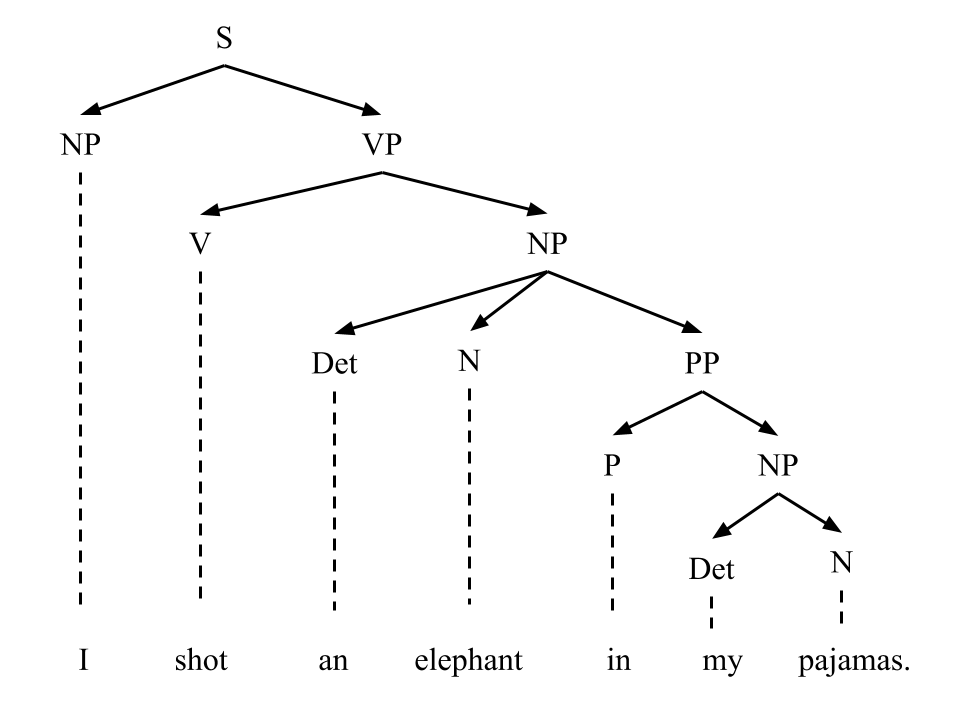
\includegraphics[width=\linewidth]{PSG_tree}
	    	\caption{Phrase Structure Grammar (PSD)}\label{fig:psg_tree}
	\end{subfigure}
	\begin{subfigure}[b]{.49\linewidth}
		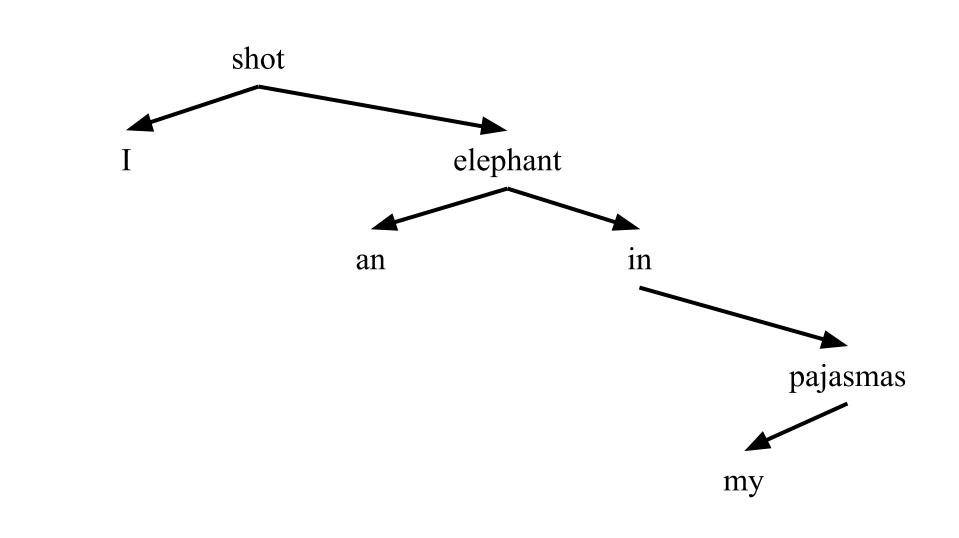
\includegraphics[width=\linewidth]{DG_tree}
		\caption{Dependency Grammar (DG)}\label{fig:dg_tree}
	\end{subfigure}
	\caption{Grammar trees examples}
	\label{fig:grm_tree_ex}
\end{figure}


\begin{figure}[h]
	\centering
	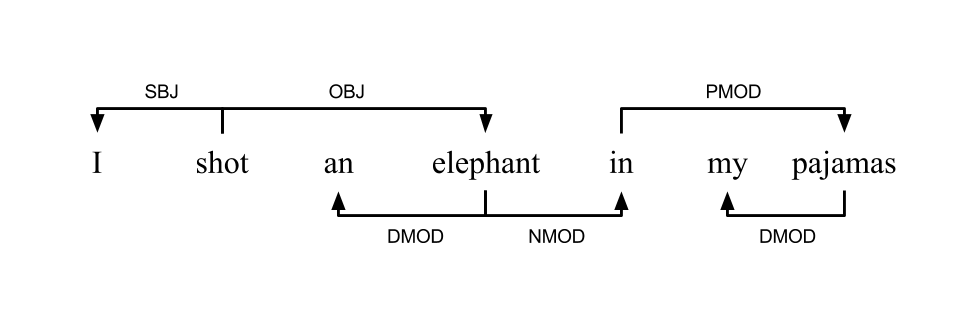
\includegraphics[width=\linewidth]{DG_tree_2}
	\caption{Dependency tree with labels}
	\label{fig:dg_tree_ex}
\end{figure}

It is important to note that Dependency Grammar is descriptive instead of being a generative system like others. However, some equivalent frameworks are introduced to solve this.

\subsection{Heads and dependants conditions} \label{head_dep}

To determine the head $H$ and dependant $D$ roles in the mentioned binary asymmetric relation $C$, \cite{zwicky1985heads} proposed the following criteria. To be precise, these criteria are not only important to Dependency Grammar, yet other frameworks which emphasise the role of syntactic heads.
\begin{enumerate}
	\item $H$ decides the syntactic category of $C$ and is able to replace the whole construction $C$
	\item $H$ decides the semantic category of $C$ and $D$ specifies $H$
	\item $H$ is obligatory while $D$ can be optional
	\item $H$ selects $D$ and specifies whether $D$ is obligatory or not
	\item The form of $D$ depends on $H$ (agreement\dots)
	\item The linear position of $D$ is specified with reference to $H$
\end{enumerate}

It is obvious that the mentioned criteria are mixture of both semantic and syntactic types (cf. criterion 1 and 2...).

By satisfying different combination of these criteria, our head-dependant relationship can be classified into various kinds of dependencies. For examples, endocentric construction refers to a construction that the head can replace the whole construction and does not destroy the structure at the same time. The relation between \textit{elephant} and \textit{in} in Figure \ref{fig:dg_tree_ex} is an example of this type. In which, \textit{elephant} can substitute the whole portion of ``elephant in my pajamas" (construction between head and dependant which includes the dependant's subordinates). The type of construction may satisfy all the criteria.

On the other hand, also in Figure \ref{fig:dg_tree_ex}, the exocentric construction between \textit{shot} and \textit{elephant} fulfils all the requirements except the first one. It is obvious that in this type of relation, by replacing the construction by head, we disrupt the whole structure, in syntactic term. The distinction that differs endocentric and exocentric is also related to the distinction between head-argument and head-modifier because, as in our examples, the head-modifier relation is endocentric while head-argument is exocentric.

In addition, there is also the third type of relation, recognised as head-specifier relation, between function words and their arguments (e.g. determiner and noun). In Figure \ref{fig:dg_tree_ex}, a clear example is \textit{an} and \textit{elephant}. This relation type is exocentric in the same way of head-argument relation. Besides the three kinds mentioned, there are also some situation that is hard to determined. For example, coordination (Tesn{\`e}re's junction) such as ``We would like to have \textit{milk and tea}", in which case determining where the head is may be impossible. The similar problems also occur in complex verb group (auxiliary and main verb), subordinate clauses and prepositional phrases\dots

\section{Dependency graphs} \label{dg_graph}
Our dependency tree in Figure \ref{fig:dg_tree} can be defined as a directed graph $G=\{V, A, <\}$ in which:
\begin{itemize}
	\item $V$ is the set of node (or vertices)
	\item $A$ is the set of arcs (or directed edges)
	\item $<$ depicts the word order on V
\end{itemize}
While nodes in $V$ are usually labelled with word forms, in the labelled version of the graph (Figure \ref{fig:dg_tree_ex}), element of set $A$ is a triple $(i,j,l)$ where $i, j \in V, l \in L$ which $L$ is the set of available arc labels.

\subsection{Formal conditions}
To capture the dependent relations between lexical items, there are some constraints on the defined graph that needs to be followed. To formally state these constraints, we need to define these following notation of graph $G$:
\begin{itemize}
	\item Node $i$ is the head of node $j$ or $i$ governs $j$ or $j$ depends on $i$
		\[i\rightarrow j \equiv \exists l\in L: (i,j,l) \in A\]
	\item Node $i$ and $j$ have a relationship:
		\[i \leftrightarrow j \equiv i\rightarrow j \vee j\rightarrow i\]
	\item Node $i$ is an ancestor of node $j$ (there exists a path from $i$ to $j$ through arcs in $G$):
		\[i\rightarrow^* j \equiv \exists i': i\rightarrow i', i'\rightarrow^* j\]
	\item Node $i$ and $j$ have a long-distance relationship ($i$ and $j$ are weakly/strongly connected)
		\[i\leftrightarrow^* j \equiv \exists i': i\leftrightarrow i', i'\leftrightarrow^* j\]
\end{itemize}

By having defined those notations, the constraints on graph $G$ can be listed as follow:
\begin{itemize}
	\item $G$ is weakly connected, i.e. there always exists an undirected path between any nodes in $G$ (connectedness)
		\[i\leftrightarrow^* j, \forall i,j\in V\]
	\item $G$ has no cycle (acyclic)
		\[\neg(i\rightarrow^* j \wedge j\rightarrow^* i), \forall i,j\in V\]
	\item Each node in $G$ has only one head (single-head)
		\[\forall i, j\in V, i\rightarrow j: \not \exists i', i\rightarrow j\]
	\item G is projective
		\[\forall i,j\in V,i\rightarrow j: i\rightarrow^* i', \forall i'\in V,i<i'<j \vee j<i'<i\]
\end{itemize}
The final condition, projectivity, can be interpreted as for any node (lexical item) that lies between head $i$ and $j$ (left arc with $j<i'<i$ or right arc with $i<i'<j$) must take $i$ as its ancestor. This is to make sure of there is no intersection between arcs when they are represented as in Figure \ref{fig:dg_tree_ex}. Please note that most theoretical frameworks do not assume projectivity which needed to denote long-distance dependencies. In addition, projectivity is not taken for granted in free-word-order languages.

\subsection{Formal properties}
Consequently, graph $G$ as defined and obeyed the constraints above holds its own properties:
\begin{itemize}
	\item Anti-symmetric: in which $\forall i,j\in V, i\rightarrow j \Rightarrow j\not\rightarrow i$
	\item Anti-reflexive: a node can be its own head $i\rightarrow j \Rightarrow i\neq j$
	\item Anti-transitive: $\forall i,j,k\in V, i\rightarrow j, j\rightarrow k \Rightarrow i\not\rightarrow k$ which means there is no direct arc from one (non-parent) ancestor to a node. This is also guaranteed by single-head condition.
\end{itemize}

\section{Variants of Dependency Grammar} \label{dg_var}

As stated in the beginning of this report, Dependency Grammar is not a single well-established framework but a varieties of frameworks that share several standard assumptions. These variants can be classified by four big open questions serve as four dimensions.

\subsection{Necessity and sufficiency}
The first question to be asked is whether dependency structure is sufficient as well as necessary. The original dependency structure of connection (as quoted from Tesn{\`e}re) does not rise this question. However, the concept of junction and transfer draw our attention in different kinds of dependency. While junction was introduced in the previous section, transfer depicts the relation between function word and the word that is being changed, in term of syntactic category.

\subsection{Mono-stratal vs. multi-stratal}
The second dimension categorises mono-stratal and multi-stratal frameworks. To be more precise, the mono-stratal framework relies on one single syntactic representation, which class includes the original theory. While multi-stratal counterparts, as most theories of Dependency Grammar, take into account several layers of representation. For example, Mean Text Theory \cite{melʹvcuk1988dependency} allows different dependency layers which are surface syntactic and deep syntactic representations. The need of the multi-layer dependency is very intuitive. Let us take the two following sentences:
\begin{minted}{text}
	I am a student.
	We are students.
\end{minted}
In traditional sense of dependency, subject depends on the main verb, as \textit{I} to \textit{am} or \textit{we} to \textit{are}. However, the form of these verbs also depend on the subjects (in case of agreement). Hence, in this case, dependence of pronouns \textit{I}, \textit{we} on the verb is syntactic, whereas, dependence of the verb (word forms) on the subjects is morphological.

\subsection{Nature of lexical elements (nodes)}
The third issue that attracts people's concern is what can be defined as the node of our dependency structure. Even though the basic assumption that the dependency relations are established between lexical elements instead of phrases (as in Phrase Structure Grammar), these elements vary between theories within the Dependency Grammar family. The original perspective assigns these nodes plainly the word forms in the sentence. Still, these nodes can be constructed by other entities such as lemmas or morphemes (in morphological dependency \cite{melʹvcuk1988dependency}).

\subsection{Nature of dependency types (arc labels)}
The fourth dimension of this variation space is the list of dependency types (i.e. arc labels such as SBJ, OBJ, NMOD\dots) employed by different theories. While some theories make use of common set of grammatical functions (e.g. subject, object\dots), the other deeper/sub-classification set (agent, patient, goal\dots)can also be used. Moreover, it is also possible to use unlabelled dependency structure, albeit not common among linguistic theories.

\section{Dependency Parsing} \label{dep_parsing}

\subsection{Deterministic parsing}
In deterministic parsing, the parser attempts to derive a syntactic representation after having processed a sequence of parsing actions. One notable incremental algorithm \cite{covington2001fundamental} links each new word to each preceding one in one single pass, with the complexity $O(n^2)$. More efficient, the shift-reduce type algorithm by \cite{nivre2003efficient} introduced three actions when parsing: shift, left-arc, right-arc. These actions are applied on a \textit{configuration} which consists of: a stack S of partially processed items, a buffer B initiated with our sentence and an empty list of relations R. Details of the actions are
\begin{itemize}
	\item Shift (SHIFT): remove a word from buffer B and push it into stack S
	\item Left-arc (LEFT): assert dependency relation between the top element of stack S and the word beneath. If true, then remove the lower word (word on top of the S is head)
	\item Right-arc (RIGHT): assert dependency relation between the second top and top element of stack S. If true, then remove the top element (word on top of the S is dependant)
\end{itemize}

Table \ref{tb:nivre_example} illustrates step-by-step actions of the algorithm. It is clearly that the algorithm runs in $O(n)$ time with a greedy strategy. The only thing left is how can our algorithm determines what action needed to be applied in a specific step. To do this, the author trained an \textit{oracle} with tree bank data to classify the required action given a configuration. Features used for this training step can be taken into consideration as word forms, part-of-speech, dependency type, etc. In general, the more features used, the better our oracle performs in term of accuracy. However, to avoid sparsity and achieve better generalisation, it is suggested to focus on most significant features at the moment of predicting (top 2 elements of the stack S...)

\begin{table}[H]
	\centering
	\begin{tabular}{c | p{4cm} | p{4cm} | p{2.8cm}}
		\textbf{Action} & \textbf{Stack} & \textbf{Buffer} & \textbf{Relations} \\
		\hline
		& [root] & [I, shot, an, elephant, in, my, pajamas] & \\
		\cline{1-3}
		SHIFT & [root, I] & [shot, an, elephant, in, my, pajamas] &\\
		\cline{1-3}
		SHIFT & [root, I, shot] & [an, elephant, in, my, pajamas] &\\
		\cline{1-3}
		LEFT & [root, shot] & [an, elephant, in, my, pajamas] & (I$\leftarrow$shot)\\
		\cline{1-3}
		SHIFT & [root, shot, an] & [elephant, in, my, pajamas] &\\
		\cline{1-3}
		SHIFT & [root, shot, an, elephant] & [in, my, pajamas] &\\
		\cline{1-3}
		LEFT & [root, shot, elephant] & [in, my, pajamas] & (an$\leftarrow$elephant)\\
		\cline{1-3}
		SHIFT & [root, shot, elephant, in] & [my, pajamas] &\\
		\cline{1-3}
		SHIFT & [root, shot, elephant, in, my] & [pajamas] &\\
		\cline{1-3}
		SHIFT & [root, shot, elephant, in, my, pajamas] & [] &\\
		\cline{1-3}
		LEFT & [root, shot, elephant, in, pajamas] & [] & (my$\leftarrow$pajamas)\\
		\cline{1-3}
		RIGHT & [root, shot, elephant, in] & [] & (in$\rightarrow$pajamas)\\
		\cline{1-3}
		RIGHT & [root, shot, elephant] & [] & (elephant$\rightarrow$in)\\
		\cline{1-3}
		RIGHT & [root, shot] & [] & (shot$\rightarrow$elephant)\\
		\cline{1-3}
		RIGHT & [root] & [] & (root$\rightarrow$shot)\\
		\hline
	\end{tabular}
	\caption{Nivre's algorithm example}
	\label{tb:nivre_example}
\end{table}

\subsection{Non-projective dependency parsing}
Nevertheless, the algorithms mentioned in previous section can only perform on projective dependency structure. Without projectivity assumption, there are two types of approaches to deal with the problem. First, one can apply specialised algorithm for non-projective dependency parsing such as a set of constraint satisfaction methods (\cite{duchier2001topological}, \cite{foth2004broad}) or graph-based algorithm by finding minimum spanning tree \cite{mcdonald2005non}. The second type is to do post-processing. This post-processing techniques generally require two steps:
\begin{enumerate}
	\item Approximate the best possible projective dependency graph.
	\item Improve our approximate solution by replacing projective arcs with non-projective arcs.
\end{enumerate}

The group of approaches include approximate non-projective parsing \cite{mcdonald2006online} or pseudo-projective parsing \cite{nivre2006labeled} in which the algorithm \textit{projectivise} the training data by providing ``projective head" (nearest permissible ancestor) instead of ``real head".

\bibliography{report}{}
\bibliographystyle{apalike}

\end{document}
